\subsection{Binning strategy for differential observables}
Choice of bin boundaries and number of bins are two important aspects of differential measurements. 
With respect to the Run 1 analyses, we are benefitted from more statistic during Run 2 where data is recorded at $137~\mathrm{fb}^{-1}$ with CMS detecor.
Sufficient statistics has helped to choose more fine binning for the observables than before. 
%For the current analysist two strategy are underway:
Bin boundaries are chosen in such a way that there is similar relative uncertainties on the expected cross section in the respective bins. Relative uncertainy ($\Delta_{rel}$) is defined as:
	%\begin{center}
\begin{equation} \label{eq:rel_unc}
	$\Delta^{i}_{rel}$ = $\frac{d\sigma^{i}_{fid}}{\Delta^{i}_{tot}}$ %(D_{\mu}\phi)^{\dag}(D_{\mu}\phi)+\mathrm{V}(\phi^{\dag}\phi)
	\end{equation}
%	\end{center}

where d$\sigma^{i}_{fid}$ and $\Delta^{i}_{tot}$ are expected cross section and total uncertainty in bin $i$ for a differential observable. 

Table \ref{tab:pTH} shows the current choice of bin boundries of $p_{T}(H)$ observables with details of expected cross section and relative uncertainties in the bins. 

\begin{table}[!h!tb]
\begin{center}
\small
\caption{
Differential cross section results for the pT4l observable.
\label{tab:pTH}
}
\begin{tabular}{|c|ccccc|} \hline \hline
Bin range (GeV) & d$\sigma_{fid}$ (fb) & $\Delta_{tot}$ (\% fb) & $\Delta_{rel}$ (\%)  & $\delta_{stat}$ (\% fb)  & $\delta_{syst}$ (\% fb) \\ \hline \hline
%\multicolumn{6}{|c|}{ \textbf{CMS preliminary choice }} \\ \hline
        0 - 10 &  0.34 &  $^{+0.11}_{-0.096}$ &  $^{+33}_{-28}$ &  $^{+0.1}_{-0.091}$ &  $^{+0.048}_{-0.031}$ \\ %0.32 &  $^{+11.01}_{-9.66}$ &  $^{+34.83}_{-30.55}$ &  $^{+10.20}_{-9.00}$ &  $^{+4.20}_{-3.40}$ \\
  10 - 20 &  0.53 &  $^{+0.13}_{-0.11}$ &  $^{+25}_{-21}$ &  $^{+0.12}_{-0.11}$ &  $^{+0.056}_{-0.037}$ \\ %0.67 &  $^{+13.98}_{-12.62}$ &  $^{+20.80}_{-18.78}$ &  $^{+12.70}_{-11.60}$ &  $^{+5.80}_{-4.90}$ \\
  20 - 30 &  0.42 &  $^{+0.11}_{-0.097}$ &  $^{+27}_{-23}$ &  $^{+0.1}_{-0.093}$ &  $^{+0.044}_{-0.027}$ \\ %0.41 &  $^{+11.77}_{-10.34}$ &  $^{+28.95}_{-25.43}$ &  $^{+10.90}_{-9.70}$ &  $^{+4.30}_{-3.50}$ \\
  30 - 45 &  0.43 &  $^{+0.11}_{-0.094}$ &  $^{+25}_{-22}$ &  $^{+0.1}_{-0.089}$ &  $^{+0.044}_{-0.029}$ \\ %0.51 &  $^{+11.72}_{-10.50}$ &  $^{+22.83}_{-20.45}$ &  $^{+10.80}_{-9.80}$ &  $^{+4.50}_{-3.80}$ \\
  45 - 80 &  0.52 &  $^{+0.11}_{-0.1}$ &  $^{+22}_{-19}$ &  $^{+0.1}_{-0.092}$ &  $^{+0.05}_{-0.038}$ \\ %0.45 &  $^{+10.46}_{-9.35}$ &  $^{+23.29}_{-20.82}$ &  $^{+9.80}_{-8.80}$ &  $^{+3.80}_{-3.20}$ \\
  80 - 120 &  0.25 &  $^{+0.073}_{-0.062}$ &  $^{+29}_{-25}$ &  $^{+0.069}_{-0.06}$ &  $^{+0.024}_{-0.018}$ \\ %0.30 &  $^{+7.72}_{-6.72}$ &  $^{+26.12}_{-22.75}$ &  $^{+7.40}_{-6.50}$ &  $^{+2.20}_{-1.80}$ \\
  120 - 200 &  0.18 &  $^{+0.057}_{-0.048}$ &  $^{+31}_{-26}$ &  $^{+0.055}_{-0.046}$ &  $^{+0.016}_{-0.011}$ \\ %0.19 &  $^{+5.74}_{-4.89}$ &  $^{+30.46}_{-25.91}$ &  $^{+5.60}_{-4.70}$ &  $^{+1.40}_{-1.20}$ \\
  200 - 13000 &  0.082 &  $^{+0.036}_{-0.028}$ &  $^{+44}_{-34}$ &  $^{+0.035}_{-0.028}$ &  $^{+0.008}_{-0.004}$ \\ %0.03 &  $^{+2.20}_{-1.50}$ &  $^{+80.48}_{-54.92}$ &  $^{+2.20}_{-1.50}$ &  $^{+0.20}_{-0.10}$ \\

\hline
%Total bins = 8 &$\sigma_{fid} = \Sigma d\sigma_{fid}$ = 2.8 (fb) & & & & &
%        \hline
%\hline
%\multicolumn{6}{|c|}{ \textbf{With ATLAS recent choice }} \\
%\hline
%
%0 - 10 &  0.35 &  $^{+11.40}_{-9.69}$ &  $^{+32.56}_{-27.67}$ &  $^{+10.30}_{-9.20}$ &  $^{+4.90}_{-3.00}$ \\
%  10 - 20 &  0.55 &  $^{+13.35}_{-11.53}$ &  $^{+24.32}_{-21.01}$ &  $^{+12.00}_{-10.90}$ &  $^{+5.90}_{-3.90}$ \\
%  20 - 30 &  0.44 &  $^{+11.41}_{-9.79}$ &  $^{+26.17}_{-22.44}$ &  $^{+10.50}_{-9.40}$ &  $^{+4.50}_{-2.80}$ \\
%  30 - 45 &  0.44 &  $^{+11.05}_{-9.54}$ &  $^{+24.97}_{-21.56}$ &  $^{+10.10}_{-9.10}$ &  $^{+4.50}_{-3.00}$ \\
%  45 - 60 &  0.29 &  $^{+8.80}_{-7.48}$ &  $^{+30.75}_{-26.14}$ &  $^{+8.30}_{-7.20}$ &  $^{+3.00}_{-2.00}$ \\
%  60 - 80 &  0.24 &  $^{+7.79}_{-6.61}$ &  $^{+31.89}_{-27.03}$ &  $^{+7.40}_{-6.40}$ &  $^{+2.50}_{-1.70}$ \\
%  80 - 120 &  0.26 &  $^{+7.33}_{-6.29}$ &  $^{+28.44}_{-24.40}$ &  $^{+7.00}_{-6.00}$ &  $^{+2.30}_{-1.80}$ \\
%  120 - 200 &  0.19 &  $^{+5.78}_{-4.85}$ &  $^{+31.03}_{-26.00}$ &  $^{+5.50}_{-4.70}$ &  $^{+1.60}_{-1.20}$ \\
%  200 - 350 &  0.07 &  $^{+3.43}_{-2.61}$ &  $^{+48.63}_{-36.95}$ &  $^{+3.40}_{-2.60}$ &  $^{+0.70}_{-0.40}$ \\
%  350 - 1000 &  0.01 &  $^{+1.68}_{-0.91}$ &  $^{+125.20}_{-67.67}$ &  $^{+1.70}_{-0.90}$ &  $^{+0.20}_{-0.00}$ \\
%
%\hline
%Total bins = 10 &$\sigma_{fid} = \Sigma d\sigma_{fid}$ = 2.84 (fb) & & & & &
\hline

\end{tabular}
\normalsize
\end{center}
\end{table}

% resolution effects is applied. Throughout this document, this procedure will be referred to as
% the unfolding procedure, and the unfolded differential distributions will be referred to as distributions at the fiducial level. 
% Currently adopted procedure is ``bin-by-bin unfolding''. This procedure for the unfolding of the detector effects from the observed distributions is the same as in Refs.~\cite{CMSH4lFiducial8TeV}~and~\cite{CMSHggFiducial8TeV}. 
%The finite efficiencies and resolution effects are encoded in a detector response matrix which describes how events migrate from a given observable bin at the fiducial level to a given bin at the reconstruction level. This matrix is diagonally dominant, with sizeable off-diagonal elements for observables involving jets.
% It is aimed we would also perform matrix inversion method as a validation tool for preceding method.
%
%Examples of the efficiency matrices for gluon fusion and VBF production can be seen in Fig.~\ref{fig:eff2d}. The matrices for the $\pt_{\rm H}$ and N(jets) observables are shown.
%
%\begin{figure}[!h]
%       \centering
%       \includegraphics[width=0.32\linewidth]{Figures/results/fiducial/2016/eff2d_ggH_powheg_JHUgen_125_pT4l_2e2mu.pdf}
%       \includegraphics[width=0.32\linewidth]{Figures/results/fiducial/2017/eff2d_ggH_powheg_JHUgen_125_pT4l_2e2mu.pdf}
%       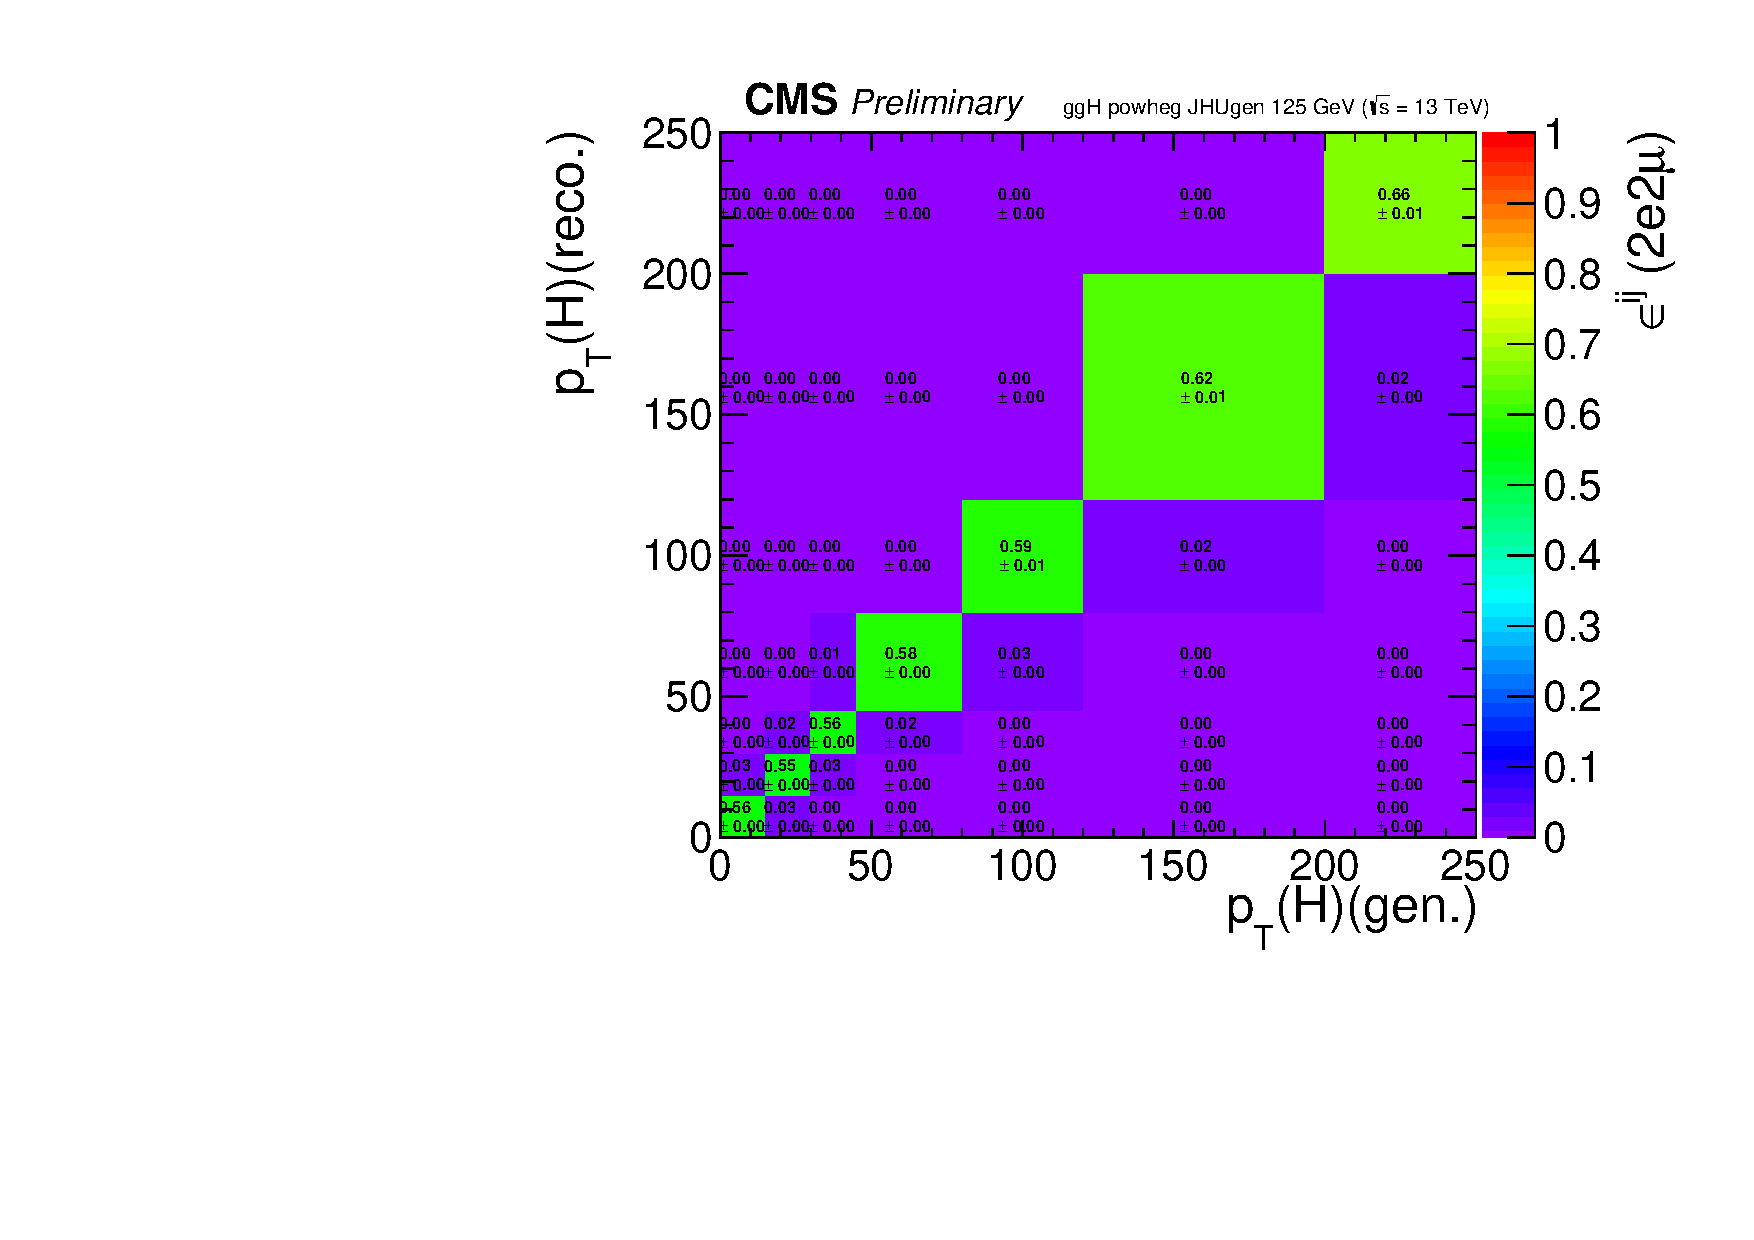
\includegraphics[width=0.32\linewidth]{Figures/results/fiducial/2018/eff2d_ggH_powheg_JHUgen_125_pT4l_2e2mu.pdf} \\
%       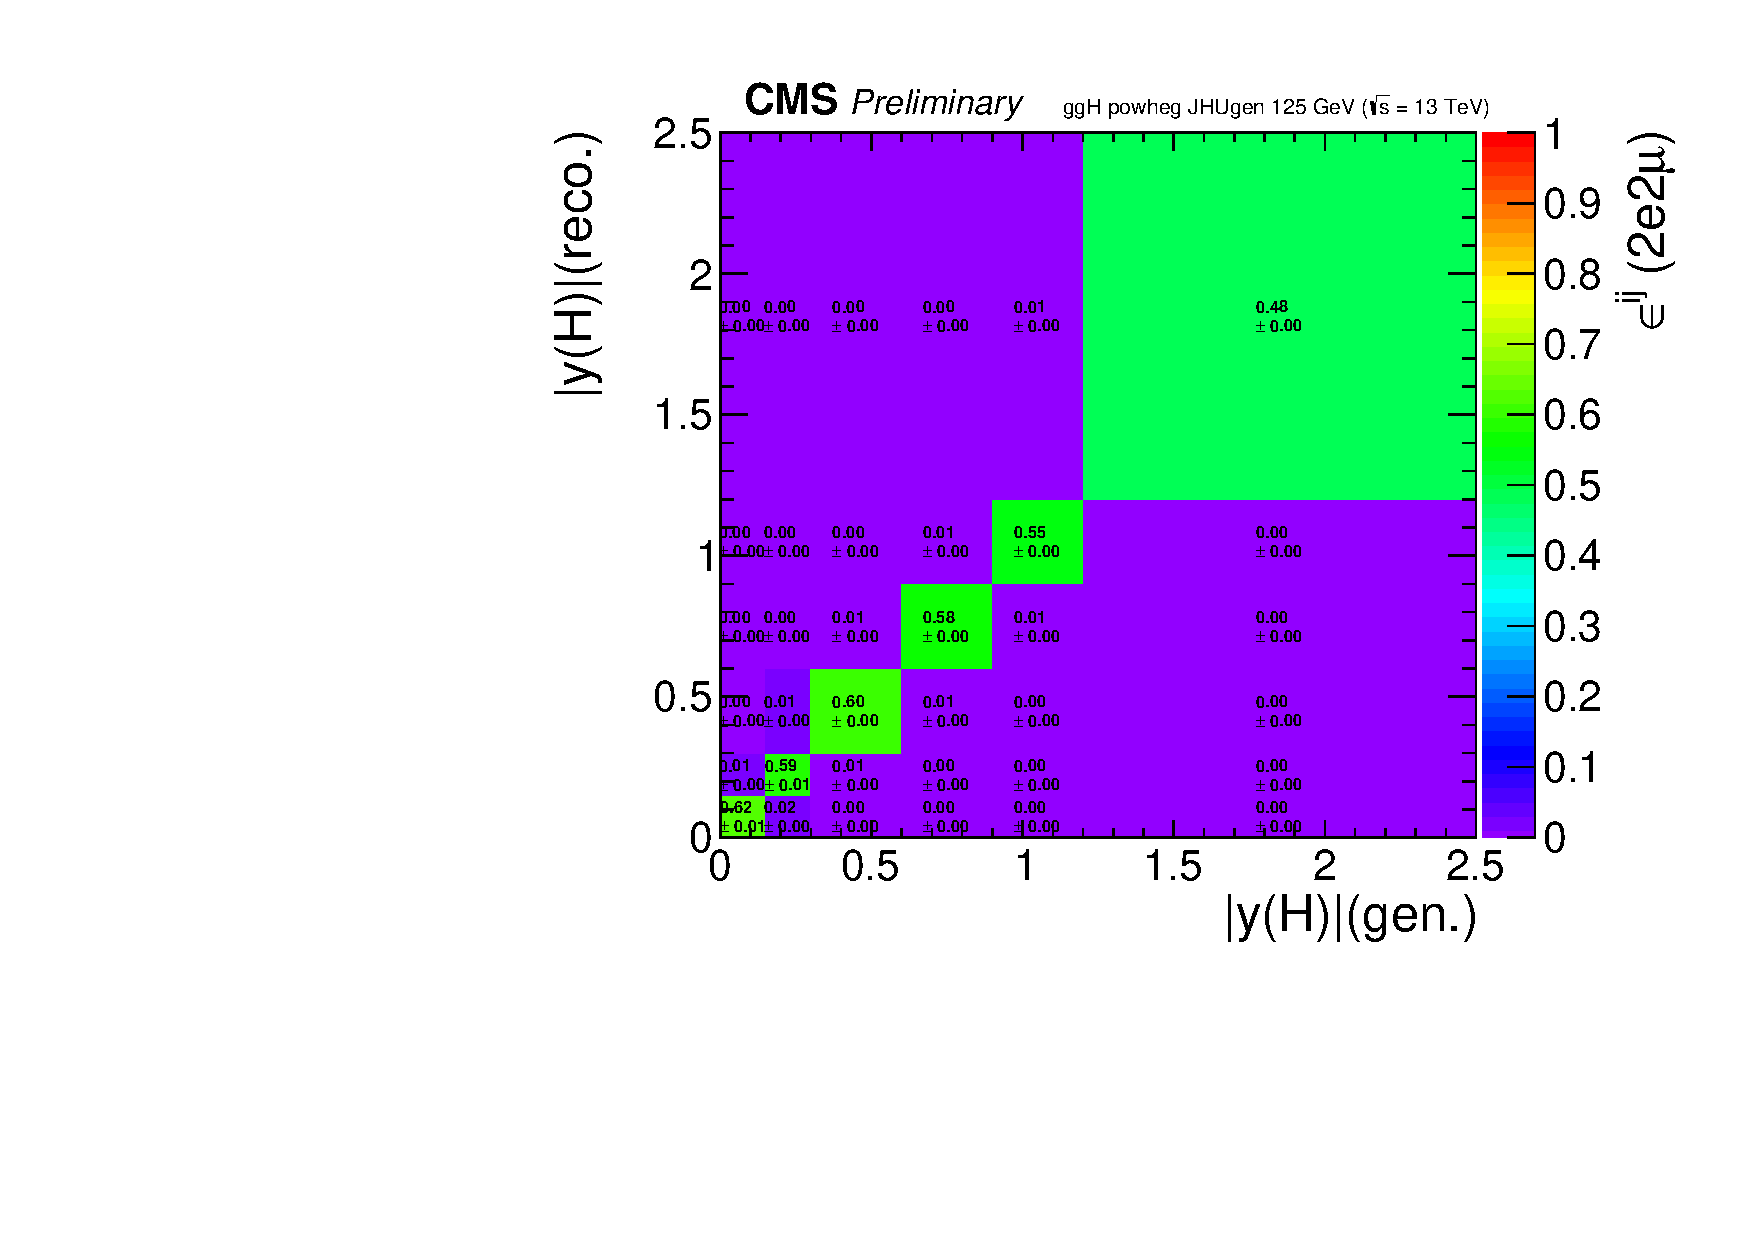
\includegraphics[width=0.32\linewidth]{Figures/results/fiducial/2016/eff2d_ggH_powheg_JHUgen_125_rapidity4l_2e2mu.pdf}
%       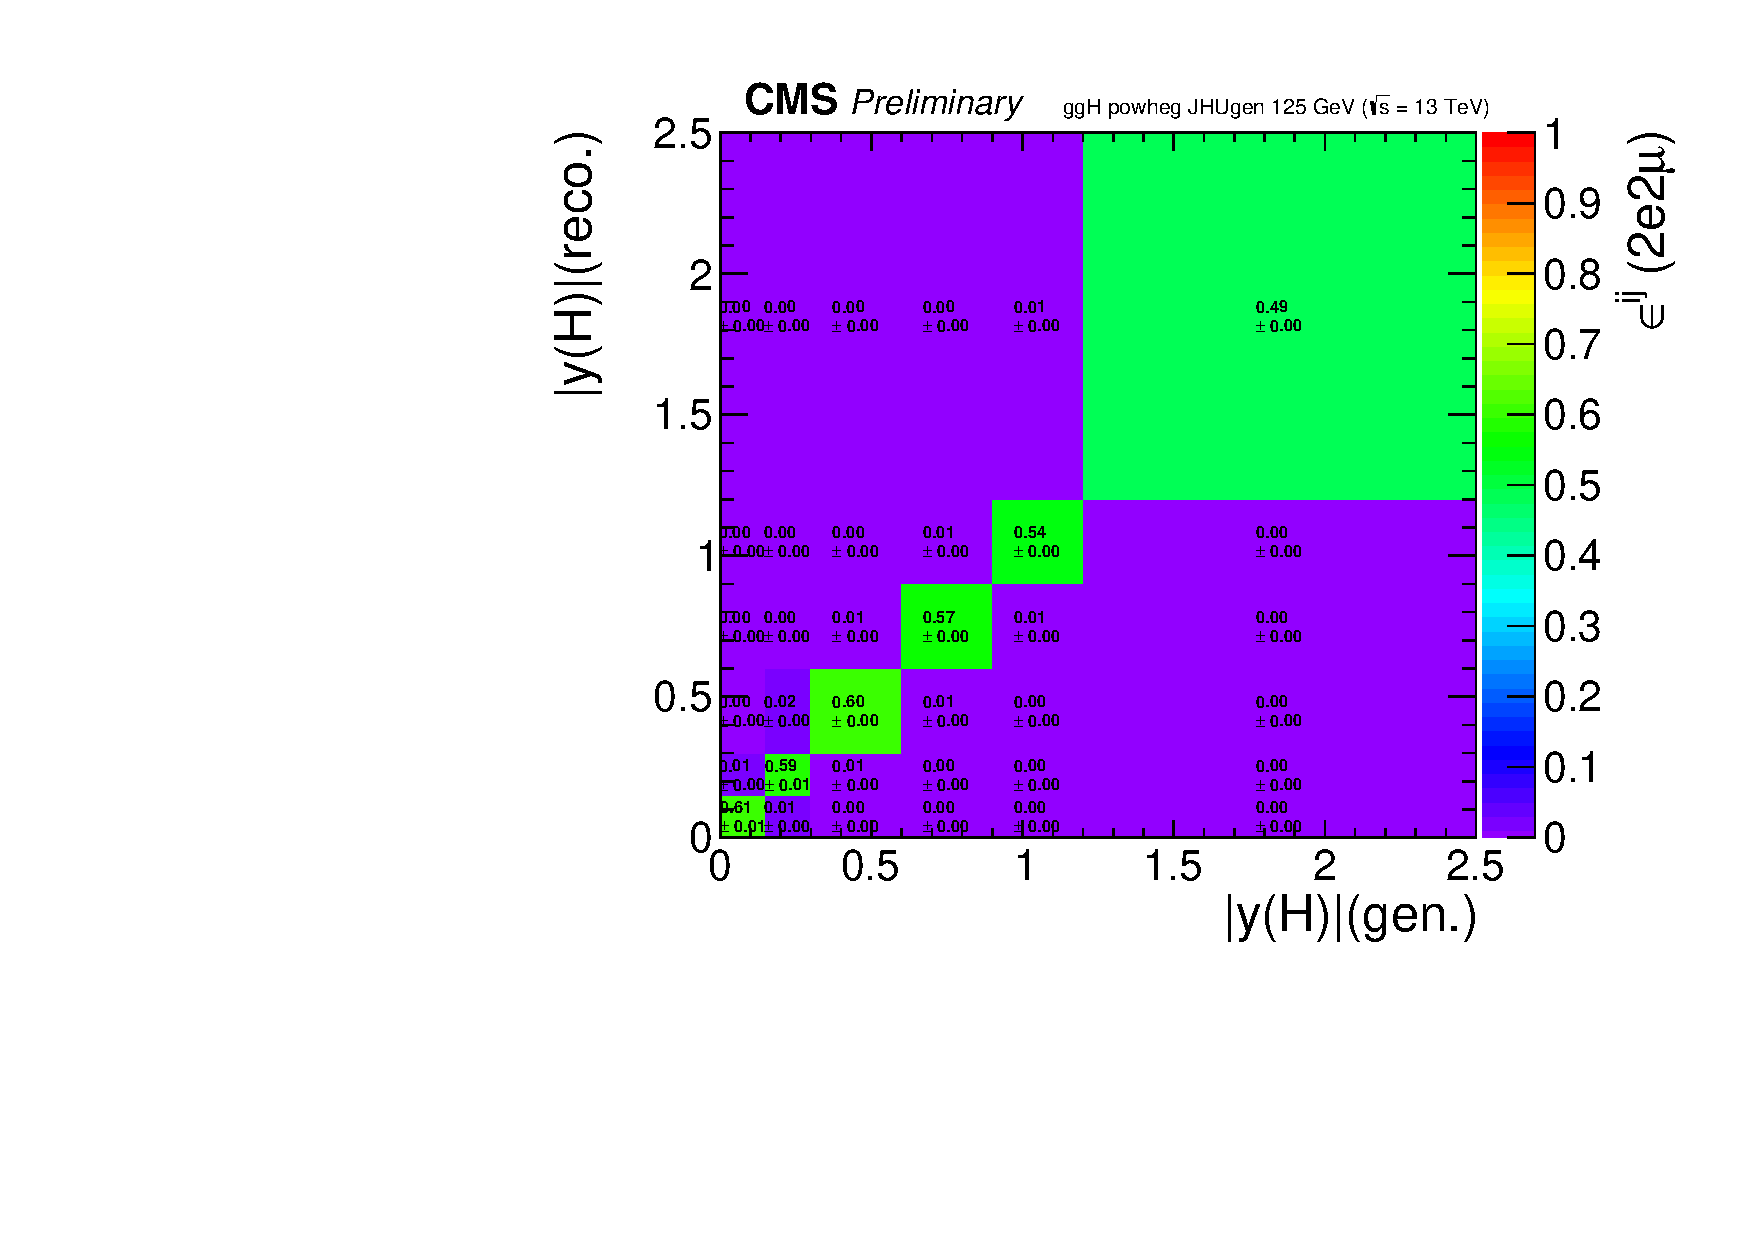
\includegraphics[width=0.32\linewidth]{Figures/results/fiducial/2017/eff2d_ggH_powheg_JHUgen_125_rapidity4l_2e2mu.pdf}
%       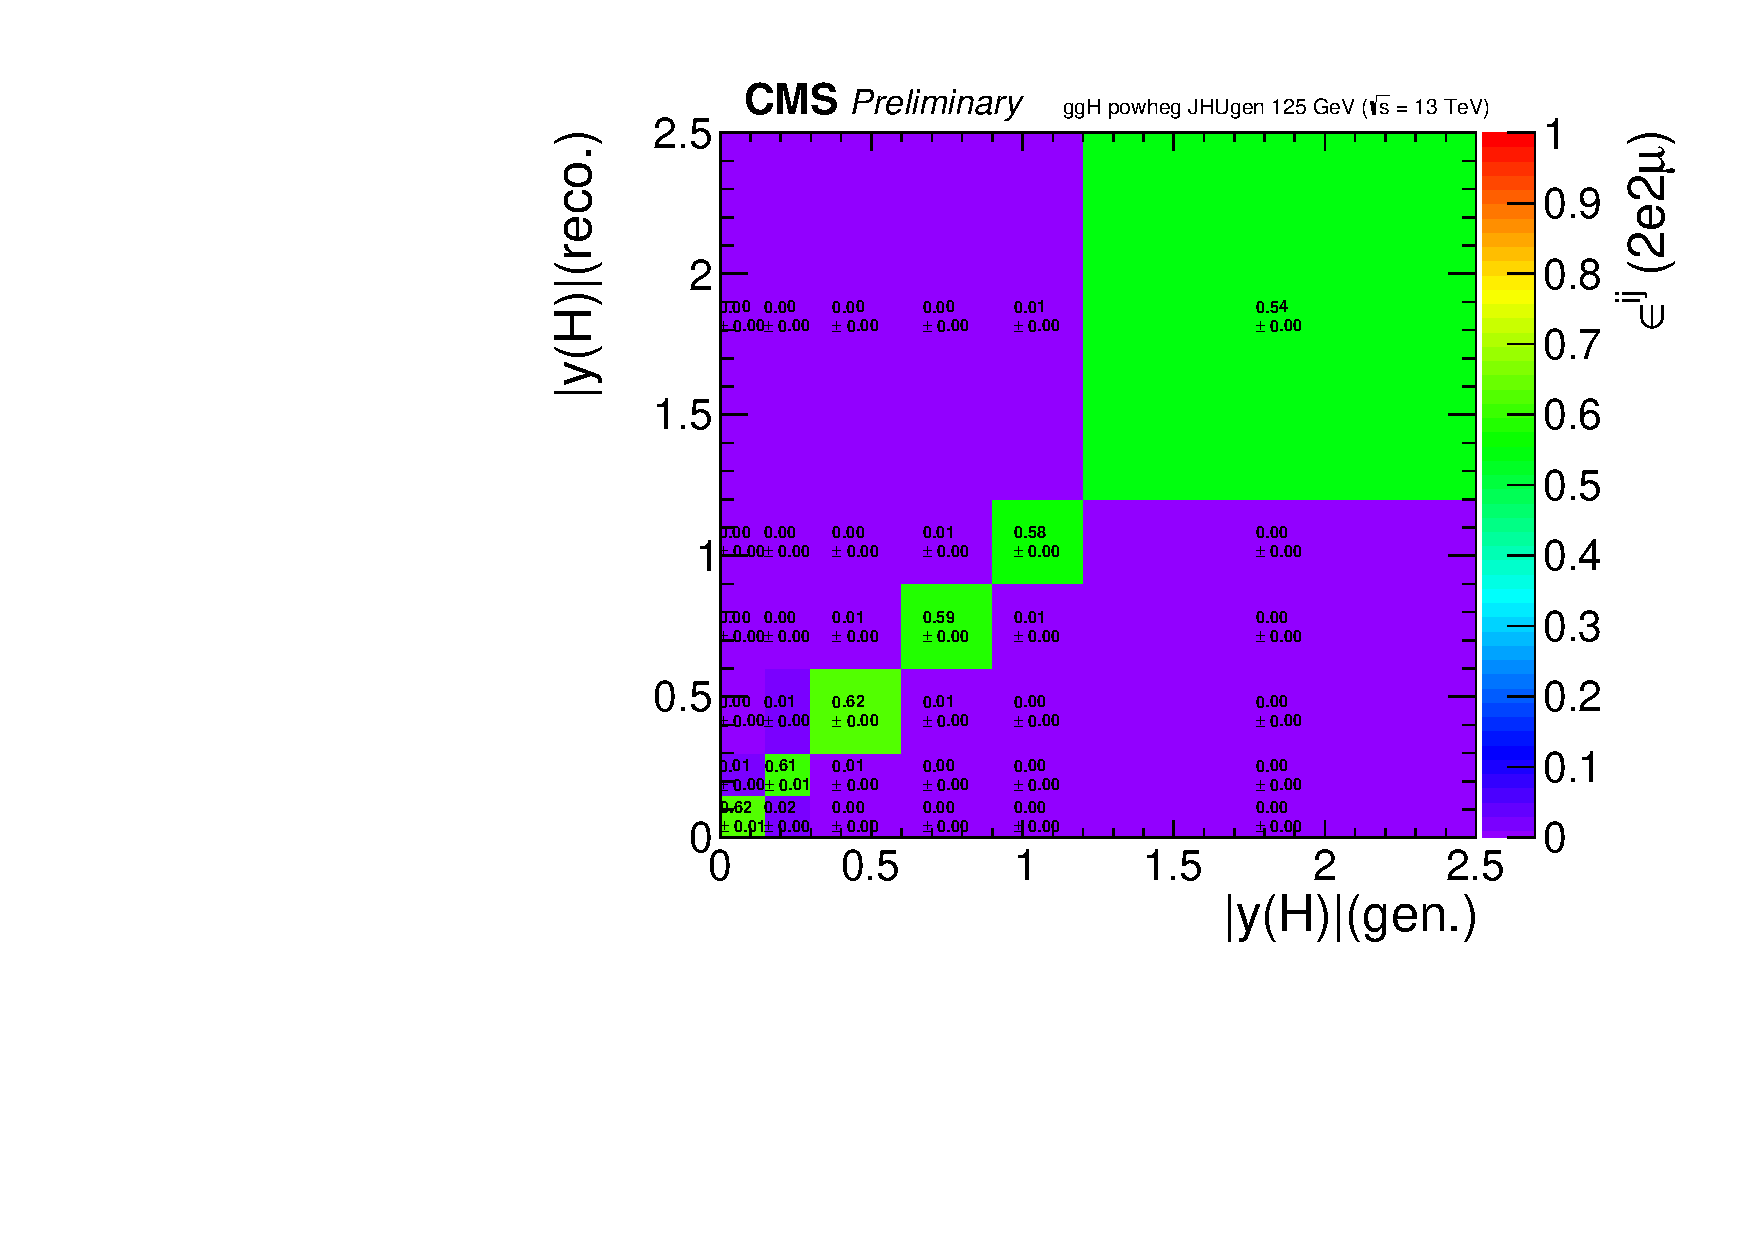
\includegraphics[width=0.32\linewidth]{Figures/results/fiducial/2018/eff2d_ggH_powheg_JHUgen_125_rapidity4l_2e2mu.pdf} \\
%       \includegraphics[width=0.32\linewidth]{Figures/results/fiducial/2016/eff2d_ggH_powheg_JHUgen_125_njets_pt30_eta2p5_2e2mu.pdf}
%       \includegraphics[width=0.32\linewidth]{Figures/results/fiducial/2017/eff2d_ggH_powheg_JHUgen_125_njets_pt30_eta2p5_2e2mu.pdf}
%       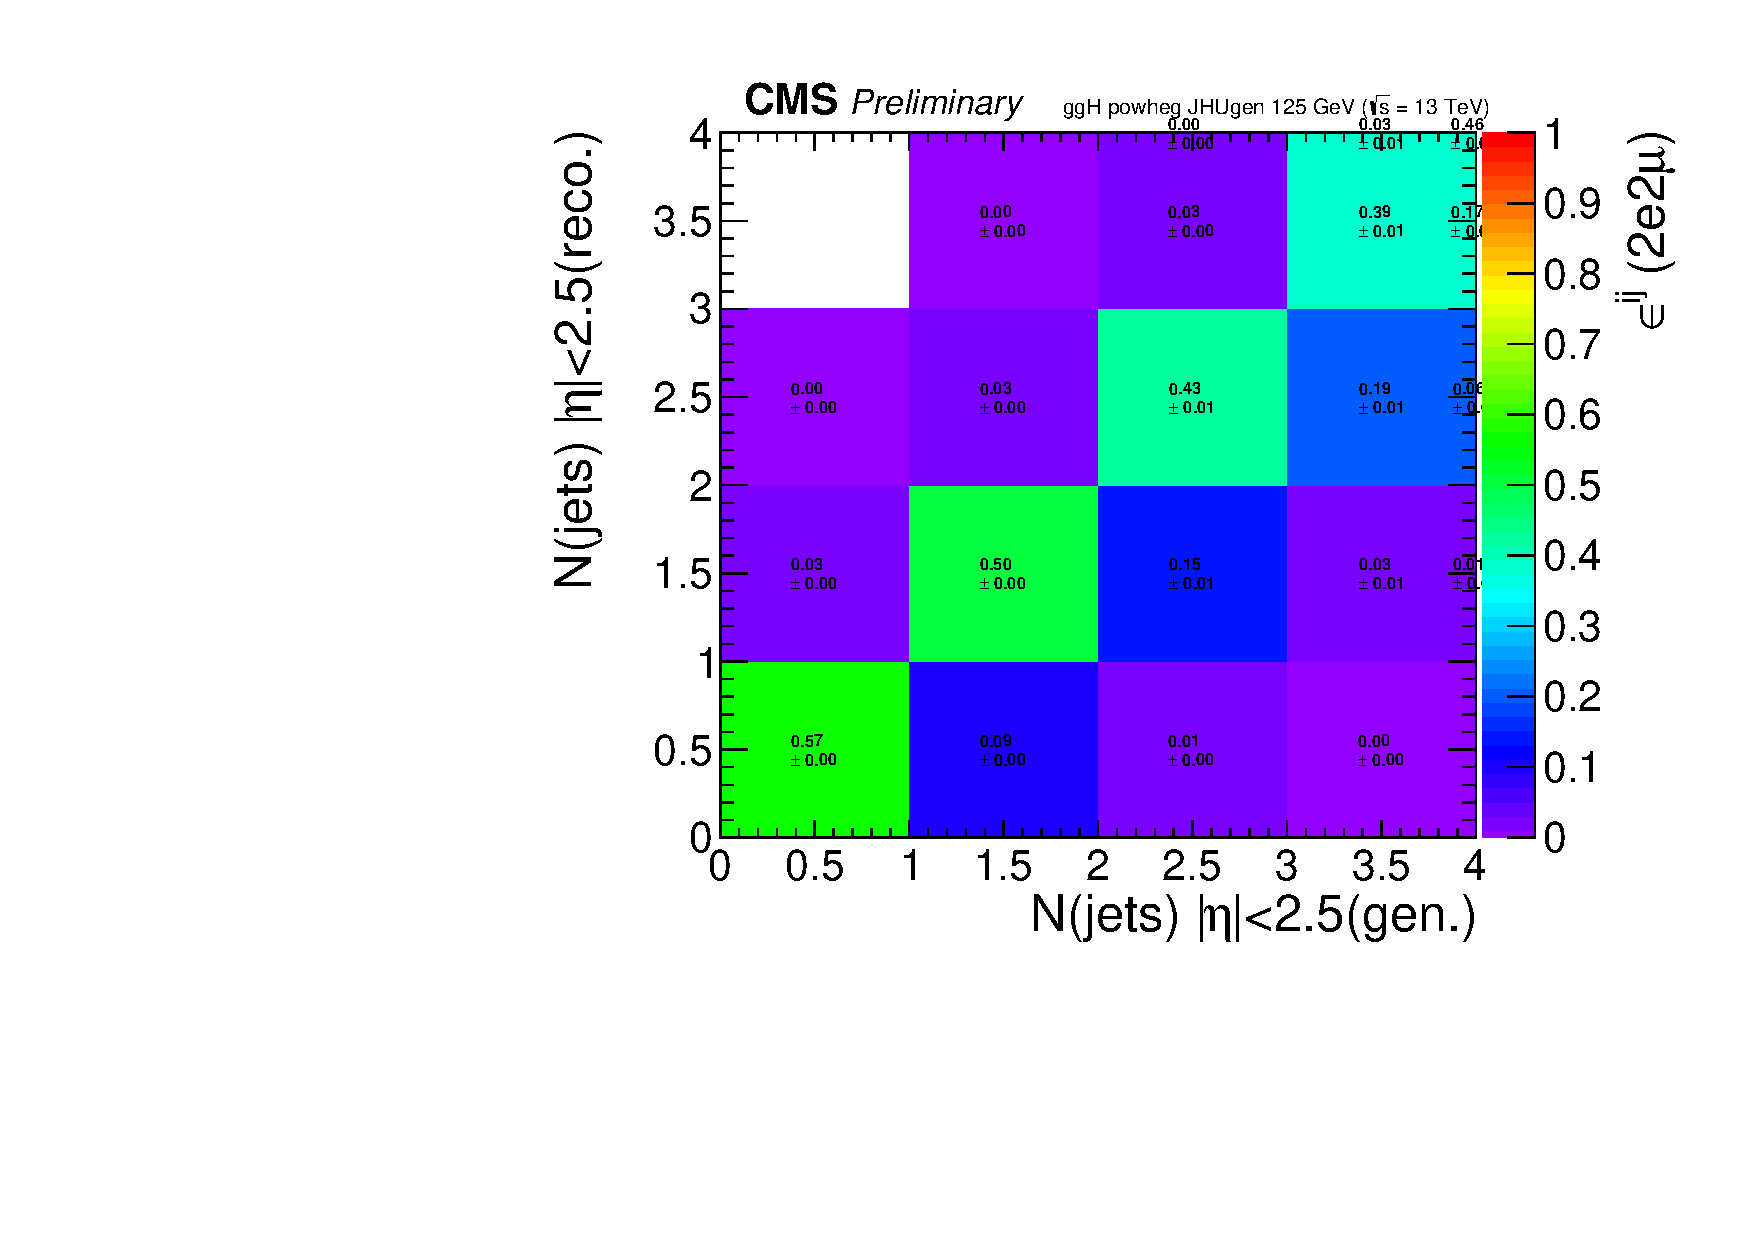
\includegraphics[width=0.32\linewidth]{Figures/results/fiducial/2018/eff2d_ggH_powheg_JHUgen_125_njets_pt30_eta2p5_2e2mu.pdf}
%
%       \caption{Efficiency matrices for the $\pt_{\rm H}$ (top) and $y{\rm H}$ (middle) and N(jets) (bottom) observables for gluon fusion production
%	       modes in the $2e2\mu$ final state in 2016 (left) 2017 (middle) and 2018 (right) (TBU). \label{fig:eff2d}}
%\end{figure}
%%The reconstruction level selection, fiducial volume definition,
%%statistical procedure, and their model dependence will be described the subsequent sections.

